
\documentclass{article}
\usepackage[letterpaper,margin=1in]{geometry}
\usepackage[utf8]{inputenc}
\usepackage{enumerate}
\usepackage{bbm}
\usepackage{mathbbol}
\usepackage[algosection,ruled,lined,linesnumbered,longend]{algorithm2e}
\usepackage{algorithmic}
\usepackage{latexsym}
\usepackage{graphicx,wrapfig,xcolor}
\usepackage{float}
\usepackage{caption}
\usepackage{subcaption}
\usepackage{amssymb}
\usepackage{amsmath,amssymb,amstext,amsthm}
%\usepackage{comment}

 \newcommand{\comment}[1]{[\begingroup\color{red!60!black}#1\endgroup]
   \marginpar{\tiny\textsc{{\color{red!60!black} To Do!}}}}

 \newcommand{\interior}{\ensuremath{\mbox{int}}} 
\newcommand{\cmd}[1]{\ensuremath{\mbox{\bf #1}}} 
\newcommand{\vio}{\ensuremath{\cmd{violation}}}
\newcommand{\st}{\ensuremath{\mbox{s.t.}}}
\newcommand{\red}[1]{\textcolor{red}{#1}}
\newcommand{\beq}{\begin{equation}}
\newcommand{\bet}{\begin{table}}
\newcommand{\eeq}{\end{equation}}
\newcommand{\real}{\mathbb{R}} %IMPORTANT
\newcommand{\htp}{\ensuremath{\mbox{HTP}}}
\newcommand{\ect}{\ensuremath{\mbox{ECT}}}
\renewcommand{\H}{\ensuremath{\mathcal{H}}}
\newcommand{\A}{\mathbb{A}}
\newcommand{\C}{\ensuremath{\mathcal{C}}}
\newcommand{\D}{\ensuremath{\mathcal{D}}}
\newcommand{\B}{\mathcal{B}}
\newcommand{\F}{\mathbb{F}}
\newcommand{\N}{\mathbb{N}} \newcommand{\R}{\mathbb{R}}
\newcommand{\T}{\mathbb{T}} \newcommand{\Z}{\mathbb{Z}}
\newcommand{\Q}{\mathbb{Q}}
\newcommand{\0}{\mathbb{0}} 
\newcommand{\1}{\mathbb{1}} 


\newtheorem{theorem}{Theorem}[section]
\newtheorem{lemma}[theorem]{Lemma}
\newtheorem{definition}[theorem]{Definition}
\newtheorem{corollary}[theorem]{Corollary}
\newtheorem{example}[theorem]{Example}
\newtheorem{nmbrs}[theorem]{Numbering}
\newtheorem{assump}[theorem]{Assumption}
\newtheorem{prop}[theorem]{Proposition}
\newtheorem{prob}[theorem]{Problem}
\newtheorem{lem}[theorem]{Lemma}
\newtheorem{thm}[theorem]{Theorem}
\newtheorem{cor}[theorem]{Corollary}
\newtheorem{rem}[theorem]{Remark}
\newtheorem{remark}[theorem]{Remark}
\newtheorem{conj}[theorem]{Conjecture}
\newtheorem{alg}[theorem]{Algorithm}
\newtheorem{ex}[theorem]{Exercise}
\newtheorem{problem}[theorem]{Problem}
\newtheorem{result}[theorem]{Result}
\newtheorem{claim}[theorem]{Claim}
\newtheorem{coroll}[theorem]{Corollary}
\newtheorem{theo}[theorem]{Theorem}
\newtheorem{defin}[theorem]{Definition}
\newtheorem{nota}[theorem]{Notation}
\newtheorem{inva}[theorem]{Invariant}

\title{Bounding the Integrality Gap of Transversal LPs}
%\author{}
%\date{May 2019}

\begin{document}

\maketitle

\section{Introduction}

Recall that a graph $H$ is a {\em minor} of $G$, if we can obtain $H$
from $G$ through a sequence of edge contractions and deletions, and
vertex deletions. In the {\em $H$-transversal} problem (\htp) one is
given a graph $G=(V,E)$, non-negative costs $c_v$, for all $v \in V$,
and a graph $H$. The goal is to find a set $S \subseteq V$ such that
$G[V\setminus S]$ has no $H$-minor.
In the following, we let $\H$
be the set of vertex subsets of $V$ whose induced subgraphs contain an
$H$-minor; i.e., $S \in \H$ iff $G[S]$ has an $H$-minor. Consider the
following natural LP relaxation of (\htp):

\begin{align}
  \min ~~ & c^Tx \tag{$\mbox{P}_{\scriptsize \htp}$}\label{lp:p} \\
  \st ~~ & x(S) \geq 1 \quad \forall S \in \H \notag \\
          & x \geq \0. \notag
\end{align}

It is not hard to see that the integrality gap of the above LP can be
large, even in special cases. For example, it is large when $H$ is a
planar graph with at least one cycle as was argued in \cite{BH+19}.
To see this, let $G$ be an $n$-vertex graph with girth $\Omega(\log n)$
and treewidth $\Omega(n)$ (e.g., certain Ramanujan graphs
\cite{Mo94}), and let $H$ be a triangle. Letting $x_v = 1/\log n$ for
all $v \in V$ is easily seen to yield a feasible solution for
\eqref{lp:p} of value $n/\log n$. On the other hand, any integral
solution for the given \htp\ instance has cost $\Omega(n)$ since
$H$-minor free graphs have treewidth $O(1)$ \cite{BH+19}. 

\section{Hitting even cycles in minor-closed graphs}

Closely related to the above is the 
{\em even-cycle transversal} problem (\ect) where
we are given a graph $G=(V,E)$, vertex costs $c_v \geq 0$ for all
$v \in V$, and where the goal is to find a min-cost set
$S \subseteq V$ such that $G[V\setminus S]$ has no even cycles. Let
\C\ be the set of even cycles in $G$. In the following, we will sometimes 
use $C \in \C$ for the set of vertices of the corresponding cycle; the meaning will be
clear from the context. 
The natural LP relaxation of \ect\ and its dual as follows:

\medskip

\hspace*{-.7cm}
\begin{minipage}{.48\textwidth}
\begin{align}
  \min ~~ & c^Tx \tag{$\mbox{P}_{\scriptsize \ect}$} \label{lp:p2} \\
  \st ~~ & x(C) \geq 1 \quad \forall C\in \C \notag \\
          & x \geq \0. \notag
\end{align}
\end{minipage}
\hspace*{1ex}
\vline
\hspace*{1ex}
\begin{minipage}{.48\textwidth}
\begin{align}
  \max ~~ & \1^Ty \tag{$\mbox{D}_{\scriptsize \ect}$} \label{lp:d2} \\
  \st ~~ & \sum_{C \in \C, v \in C} y_C \leq c_v \quad \forall v \in V
           \notag \\
          & y \geq \0. \notag
\end{align}
\end{minipage}
\medskip

Similar to the previous argument, we can show that \eqref{lp:p2} has
an integrality gap of $\Omega(\log n)$ in general. 
We suspect, however, that the LP has integrality gap $O(1)$ when $G$ is from a
minor-closed class of graphs. We will now show this for the special
case where $c=\1$. We need the following result due to Fomin, Saurabh,
and Thilikos \cite{FST11}.

\begin{theorem}\label{thm:fst}
  Let $\mathcal{G}$ be a proper minor-closed graph class and let $H$ be
  a planar graph. Then there is
  \begin{itemize}
  \item a feasible solution $U \subseteq V$ to \htp\ for $G$ and $H$, and
  \item a collection $\cal{U}$ of pairwise
    disjoint vertex subsets of $V$ each of which induces a subgraph of
    $G$ with an $H$-minor,
  \end{itemize}
  and $|U| \leq c|{\cal U}|$ for some constant $c({\cal G},H)$.
\end{theorem}

We apply Theorem \ref{thm:fst} to the given graph $G$ from some
minor-closed graph class (e.g., planar), and choose $H$ as 
the graph on two vertices with three parallel edges. The theorem
provides us with disjoint sets of vertices $D_1, \ldots, D_p$ such
that $H$ is a minor in $G[D_i]$, for all $i \in [p]$, and a set $U$ of
vertices such that $G[V\setminus U]$ has no $H$ minor. We furthermore
know that $|H| \leq cp$ for some constant $c$.

Note that $G[D_i]$ contains an $H$-minor, and hence there are vertices
$v_i$ and $u_i$ in $D_i$, and $G[D_i]$ contains three internally
vertex-disjoint $v_i, u_i$-paths. Clearly, some two of these paths
together form an even cycle $C_i$. We conclude that letting
$y_{C_i}=1$ for all $i \in [p]$ yields a feasible solution for
\eqref{lp:d2}. It is clear that $U$ may not be a feasible even cycle
transversal in $G$. 

Recall that a {\em block} in $G$ is an inclusion-wise maximal subgraph
that is either a single vertex, a bridge-edge, or a $2$-vertex
connected subgraph. We then note that $G':=G[V\setminus U]$ is
$H$-minor free, and thus a {\em cactus}; i.e., a graph in which every
block is a simple cycle, or an edge. The {\em block graph} of $G'$ is
an acyclic bipartite graph with vertex set $B_1 \cup B_2$, where $B_2$
are the blocks of $G'$, and $B_1$ are the cut-vertices. The block
graph has an edge connecting each cut vertex with any of its incident
blocks.
Let $B'_2 \subseteq B_2$ be the set of block vertices
that correspond to {\em even} cycles of $G'$. Also let $B'_1 \subseteq B_1$ be
the cut vertices with at least two neighbours in $B'_2$.  Let $\B$ be
the subgraph of the block-graph induced by the vertices in
$B'_1 \cup B'_2$. $\B$ is a forest, and we let $T_1, \ldots, T_l$ be
its trees. Let $V(T_i)=B'_{i,1} \cup B'_{i,2}$ such that $B'_{i,q}
\subseteq B'_q$ for all $i \in [l]$, and $q \in \{1,2\}$. 

W.l.o.g., we assume that $T_1,.., T_j$ are those trees in $\B$ that
have only a single node from $B'_2$ (if no such tree exists, we let $j=0$). 
For $T_i$ with $i>j$ choose a root $r \in B'_{i,1}$
and direct the edges of $T_i$ away from $r$. For each node
$a \in B'_{i,1}$, let $b(a) \in B'_{i,2}$ be an arbitrary descendant
of $a$ in $T_i$ (such a node exists by the definition of $B'_1$). 

In the following, we abuse notation mildly, and use $b(a)$, for some
$a \in B'_{i,1}$, in place of the even cycle it represents in $G'$.
We define a feasible solution $\bar{y}$ for \eqref{lp:d2} by first letting
$\bar{y}_{b(a)}=1/2$ for all $a \in B'_{j+1,1} \cup \ldots \cup B'_{l,1}$.
For $i \in \{1, \ldots, j\}$, let $C_i$ be the even cycle
corresponding to the single $B'_2$-node in $T_i$. We then let
$\bar{y}_{C_i}=1$, for all $i \in \{1, \ldots, j\}$. 
Let $\bar{y}_C=0$ for  all other even cycles. We claim that the $\bar{y}$
constructed is feasible for \eqref{lp:d2}. 
To see this, note that, by construction, no node $v \in V(G')$ is
incident to more than two even cycles with positive $\bar{y}$ value. 
In fact, if $v$ is incident to two even cycles $C_1$ and $C_2$ with
positive $\bar{y}$ value, then $\bar{y}_{C_1}=\bar{y}_{C_2}=1/2$. 

For each $1 \leq i \leq j$, let $a_i$ be an arbitrary vertex of
$C_i$. Define
\[ \bar{U} = \{a_1, \ldots, a_j\} \cup \{ a \in B'_{j+1,1} \cup \ldots
  \cup B'_{l,1} \,:\, \bar{y}_{b(a)}>0\}, \]
and note that $U \cup \bar{U}$ is a feasible solution for the
even-cycle transversal problem. Thus, letting $x_v=1$ for all $v \in U
\cup \bar{U}$, and $x_v=0$, otherwise, yields a feasible solution to
\eqref{lp:p2}. The value of this solution is no more than
$\max\{c,2\}$ times the
value of the feasible solution $y+\bar{y}$ for \eqref{lp:d2}. 
We obtain the following result.

\begin{theorem}
  Let $G$ be chosen from some minor-closed family of graphs. Then
  \eqref{lp:p2} has a constant integrality gap. 
\end{theorem}

\section{Even cycles in planar graphs}

In this section, we provide a constant-factor gap for \eqref{lp:p2} in
planar graphs in the case of general vertex costs. We will accomplish
this by refining the argument given in \cite{FJP10} for the case of
hitting {\em diamonds}.

A diamond is any sub-division of the graph consisting of three
parallel edges. In \cite{FJP10}, Fiorini et al. consider the problem
of finding a minimum-cost diamond-transversal in a general graph. The
authors show that the natural covering LP obtained from \eqref{lp:p2}
by replacing \C\ by the set \D\ of vertex sets of diamonds in $G$ has
an integrality gap of $\Omega(\log n)$. The proof is constructive and uses
a primal-dual algorithm using the natural LP and its dual.

The algorithm in \cite{FJP10} is natural and follows the well-known
primal-dual strategy: start with a pair $x=y=\0$ of infeasible primal,
and feasible dual solution. The algorithm iteratively modifies $x$,
and $y$, maintaining the fact that $x$ is $0,1$, and $y$ is dual
feasible, and stops as soon as $x$ is primal feasible. After applying
a customary {\em reverse delete} step, the algorithm arrives at a
minimally feasible solution $\bar{x} \leq x$, and the authors show
that its total cost is bounded by $O(\log n)$ times the value of dual
solution $y$. 

Somewhat more specifically, in every step of the algorithm, where $x$
is primal infeasible, we let $X$ be the vertex set corresponding to
$x$. The algorithm then carefully chooses a diamond $D$ in
$G[V\setminus X]$, and increases its dual variable $y_D$ as much as
possible, maintaining dual feasibility. At this point, the dual packing
constraint for a vertex $v \in V\setminus X$ becomes tight, and the
algorithm sets $x_v=1$. Once $x$ is feasible for the LP, the algorithm
computes a {\em minimal} feasible solution $\bar{x} \leq x$, and the
authors show that $y_D > 0$ only if $|D \cap \bar{X}| =  O(\log
n)$. This suffices to prove that $\bar{X}$ is an $O(\log
n)$-approximate diamond hitting set. 

In this
section, we show that their algorithm can be simplified in the case of
even cycles, and that it can be strengthened using the planarity of
the underlying graph.

\subsection{Ideas and a first attempt}

A key first observation is captured in the following Lemma which is a
special case of Kotzig's Theorem on Light Planar Subgraphs (e.g., see
Section 3 of \cite{JV13}). 
Let us call a vertex \emph{heavy} if it has degree 6 or more and \emph{light} otherwise.
\begin{lemma}\label{discharge}
  A planar multigraph $ G=(V,E)$ where every vertex has at least 3
  distinct neighbours and no face of length 2 contains either
  i) a vertex of degree at most 10 which is adjacent to a vertex of degree 3, or \\
  ii) 2 vertices whose degrees sum to at most 11. Further, this bound is tight.
\end{lemma}
\begin{proof}
% starting the proof with edge max counterex
 Assume $ G=(V,E)$ is an \emph{edge maximal counterexample}. Define  $d(v)$ as the degree of $v$ in $G$. So G has minimum degree at least three and the sum of the degrees of the endpoints of every edge is strictly greater than $ 13$. The choice of $G$ implies that if there are any non-adjacent $u$ and $v$ with $d(u)+d(v)>13$, then $G+uv$ is not planar. Now we assign a \emph{charge} of charge $6-d(v)$ to each vertex $v$. The total charge is $\sum_v (6-d(v)) $ which is $   6|V| -2|E| $, which is at least 12 using the fact that $|E| \leq 3|V|- 6$ by Euler's formula.
 
 % explain discharging and positive charge
  Now we \emph{discharge}: a vertex $v$ with a positive charge distributes its charge evenly among its neighbours. To clarify, the charge is sent evenly along all edges incident to $v$. If a neighbour is connected to $v$ by multiple edges, then it gets additional charge for every edge. Since no charge is lost, there must still be vertices with a positive charge. Let $v$ be a vertex with a positive charge. So $v$ has a light neighbour. If $v$ is light, then $v$ and  a light neighbour of $v$ form a pair of vertices whose degrees sum to less than 11. So let us assume $v$ is heavy.
  
 \begin{figure}
  \begin{center}
   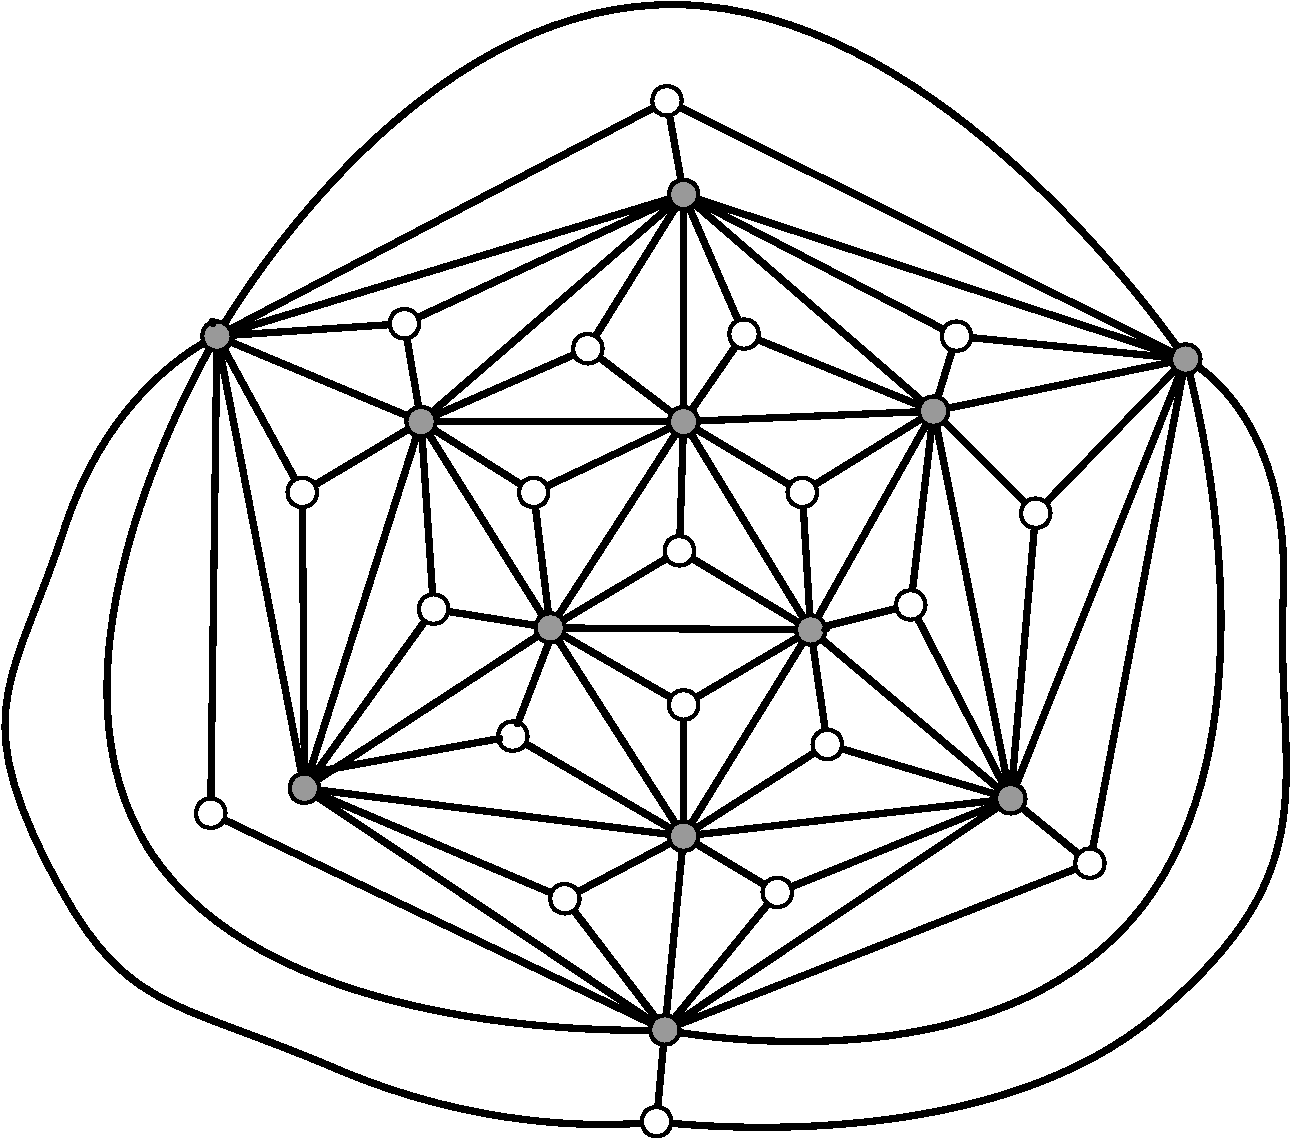
\includegraphics[width=0.39\textwidth]{StellatedIcosehedron.pdf}
   \end{center}
   \caption{\label{StellatedIco} The figure shows a {\em stellated} icosahedron for which the bound given in
   Lemma \ref{discharge} is tight.}
 \end{figure}

 %finishing the discharging argument
 Let $u_1,u_2,..,u_l$ be the neighbours of $v$ in clockwise order and let $u_{l+1}=u_1$. We claim that $u_i,u_{i+1}$ cannot both have degrees less than 6. For the sake of contradiction assume that this is not true, then $ u_i,v,u_{i+1} $ are contained in a single face $f$, and $u_i,u_{i+1}$ are not neighbours. Let $w$ be the other neighbour of $u_i$ in $f$; since $G$ contains no adjacent light neighbours, $w$ is heavy. So adding an edge between $v,w$ inside $f$ would not create adjacent vertices whose degrees sum to less than 11 nor create a face of length 2, which contradicts our choice of $G$.  Thus $v$ does not have 2 consecutive light neighbours, and so has at most as many light neighbours as heavy neighbours.  Let $l$ and $h$ be the number of light and heavy neighbours of $v$. Suppose $v$ has a neighbour $u$ of degree 3. 
 
 Vertex $v$ starts with charge at most $6-l-h$ and it receives charge at most 1 from each light neighbour and none from heavy neighbours. So the charge of $v$ is at most  $6-l-h +l =6 -h $.  So v has at most 5 heavy neighbours and hence at most 10 neighbours. Since $v$ is adjacent to $u$ which has degree 3, this proves the lemma. 
 
 %So  $u$ and $v$ form adjacent vertices whose degrees sum to at most 13. 
 For the next case, suppose $v$ has no neighbour of degree of exactly 3, and some neighbour $u$ of degree 4.  A vertex of degree 4 or more sends a charge of at most 0.5. Therefore $v$ has charge at most $ 6-l-h +0.5l $.   So the charge of $v$, which is positive, is at most $ 6-0.5l-h $, which is at most  $6- 0.75(h+l) $. Hence $v$ has degree at most 7. Consequently, $v,u$ are a pair of adjacent vertices whose degrees sum to at most 11. 
 
 If neither of the previous assumptions hold, then all the light neighbours of $v$ have degree 5. Then $v$ has charge at most $ 6-l-h +0.2l $ which is at most $6-0.9(h+l) $. Because the charge is positive, $v$ has degree at most 6. Let $u$ be any light neighbour of $v$, then $u$ and $v$ are a pair of adjacent vertices whose degrees sum to at most 11.
 \end{proof}


Lemma \ref{discharge} is indeed tight, and there are example graphs satisfying the stated conditions for which
no pair of adjacent vertices has degree sum less than 13. One such example is the {\em stellated icosahedron}
shown in Figure \ref{StellatedIco}. The above proof of Lemma \ref{discharge} provides a quite precise
characterization of tight instances $G$ satisfying the Lemma's conditions. Let $u, v$ be two adjacent vertices
whose degree sum to $13$ in such a graph $G$, and suppose, w.l.o.g., that $v$ has degree no smaller than that
of $u$. Then the above proof shows that $v$ has degree $10$ and $u$ has degree $3$. Moreover, light and heavy
neighbours of $v$ alternate, and at least $4$ of the light neighbours of $v$ must have degree exactly $3$. 

There is even more structure! Tightness of Lemma \ref{discharge} also implies that $G$ must be an edge-maximal
counter-example. Consider a face $f$ incident to $v$ containing a light neighbour $v'$ of $v$. 
Let $u'$ be the other neighbour of $v$ on the same face. Since light and heavy neighbours of $v$
alternate, $u'$ must be a heavy neighbour. We argue that $f$ must be a face of length $3$. If not, then $v'$
has a neighbour $w$ on $f$ different from $v$ and $u'$. This node $u'$ must be heavy, and hence we would be
able to add edge $vw$ to $G$ without violating planarity. A contradiction to $G$'s maximality. This shows that
all faces incident to $v$ have length $3$. 
In the following, we call a vertex $v$ {\em particular} if it has degree $10$, its neighbours are alternating
light and heavy, and all its incident faces have length $3$. 
  

Denote the dual of a graph $G$ embedded in the plane by $G^*$.   

In particular, the above lemma has the following consequence:

\begin{cor}\label{cor:smallec}
  A 2 connected planar graph G of minimum degree 3 and no face of
  length 2 contains an even cycle with at most 11 edges.
\end{cor}
\begin{proof}
By lemma \ref{discharge}, there are 2 faces $f_1,f_2 \subset E$ of $G$ whose total length is at most 13. If either $f_1,f_2$ is even it is an even cycle with at most 10 edges. Otherwise,  $f_1 \Delta f_2$ is an even cycle with at most 11 edges.
\end{proof}


\begin{figure}
  \begin{center}
    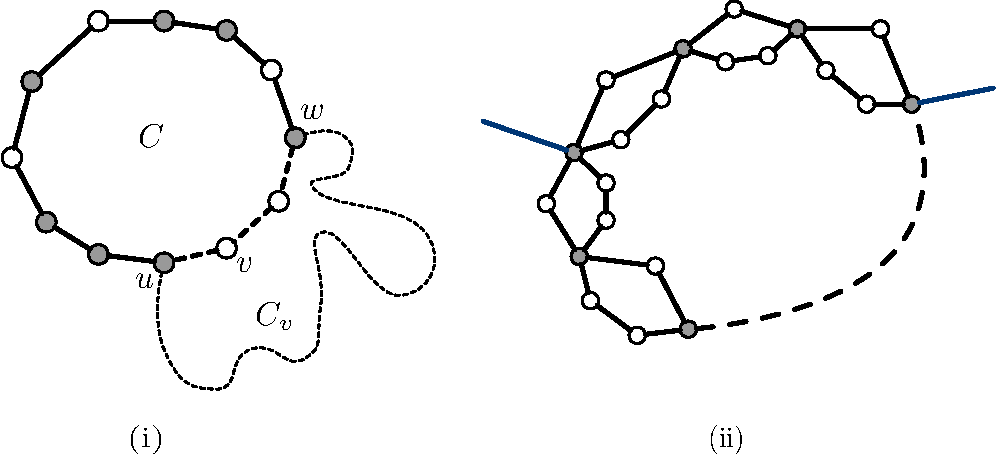
\includegraphics[width=.9\textwidth]{simple-pd.pdf}
  \end{center}
  \caption{\label{fig:simplepd} Figure (i) shows even cycle
    $C$. White vertices are contracted during compression and have
    degree 2 in $G[V\setminus X]$, grey vertices have degree at least
    3 in the same graph. Figure (ii) shows a graph in which every even cycle is long. }
\end{figure}

Hao's notes have a self-contained proof of the above two statements.
From here, our algorithm follows the ideas provided in \cite{FJP10},
simplifying and adapting to even cycles where possible. 

Corollary \ref{cor:smallec} suggests the following natural algorithm:
start with $X=\emptyset$, and $y=\0$. At any point in the algorithm
where $X$ is not feasible, compute the {\em 1-compression} $G_1$ of
$G[V\setminus X]$ as follows: as long as $G$ has a node $v$ of degree 2 with
exactly two neighbours $u$ and $w$ in $G$, {\em contract} $v$; i.e.,
replace $uv$ and $vw$ by $uw$, and delete $v$. In the resulting graph
$G_1$, all nodes have degree at least $3$. Now find a cycle $C_1$ in
$G_1$ of length at most $11$ whose corresponding cycle $C$ in $G$
(which we will also call the {\em projection} of $C_1$ in $G$)
is
even. Increase $y_C$ as much as possible, and add the newly tight
vertices to $X$. Repeat the above until $X$ is feasible, then run
reverse delete, and obtain a minimally feasible set $\bar{X}$. Note
that the minimality of $\bar{X}$ implies that, for all
$v \in \bar{X}$, there is an even {\em witness} cycle $C_v$ in $G$
that that $C_v \cap \bar{X} = \{v\}$. More precisely,  there is such a
witness cycle $C_v$ that is in the projection of  the compressed
residual graph {\em at the time} when $v$ was chosen. 

\begin{lemma} \label{lem:simplealg}
  Suppose that the above algorithm terminates with
  feasible solution $\bar{X}$. Then the total cost of $\bar{X}$ is at
  most $11$ times the value of the computed dual solution.
\end{lemma}
\begin{proof}
  Let us consider an even cycle $C$ with $y_C>0$, and let $C_1$ be the
  short cycle in the 1-compression $G_1$ of the graph $G[V\setminus
  X]$ at the time where $y_C$ was increased. 
  In Figure
  \ref{fig:simplepd}.(i), white nodes have degree $2$ in $G[V\setminus
  X]$, and grey nodes have degree at least three. Hence the cycle
  depicted has length $7$ in $G_1$. Suppose that $v \in V(C) \cap
  \bar{X}$ is a node on $C$ that was chosen by our algorithm for the
  final transversal.

  Consider two adjacent nodes $u$ and $w$ in $V(C_1)$, and let
  $P_{uw}$ be the corresponding path in $G$. 
  Let us first assume that $v$ is an internal (degree $2$) node of
  $P_{uw}$ for two adjacent nodes $u,w$ of $V(C_1)$. In this case,
  note that the witness cycle $C_v$ of $v$ contains all nodes of
  $P_{uw}$ including $u$ and $w$ themselves. Thus, if $\bar{X}$
  contains $v$ then it contains no other nodes from $P_{uw}$.

  Now suppose that $v \in \bar{X} \cap C_1$ is node of
  degree at least three on $C$, and let $u$ and $w$ be the neighbours
  of $v$ on $C_1$. Using the same argument as before, we see that
  no internal vertex of $P_{uv}$ and $P_{wv}$ can be in $\bar{X}$ in
  this case. Hence, we must have
  $|\bar{X} \cap C| \leq 11$, and the solution
  $\bar{X}$ has cost no more than $11\sum_Cy_C$. 
\end{proof}

Unfortunately, the above algorithm does not always terminate. The
reason is that we may not be able to find an even cycle whose
1-compression has at most 11 edges. Consider for example the 
graph depicted in Figure \ref{fig:simplepd}.(ii). This graph has many even
cycles, albeit no short ones! Notice that the compression of this
graph has faces of length $2$, and hence Corollary \ref{cor:smallec}
does not apply. 

\subsection{Dealing with graphs without even cycles of small
  compressed length}

Consider vertex sets $C'_1$ and $C'_2$ that each contain the  vertex set of an even cycle
in $G$; i.e., for $j \in \{1,2\}$, there is an even cycle $C_j \in \C$ such that $C_j
\subseteq C'_j$. 
Define $a_v^{C'_1,C'_2}=1$
for all $v \in (C'_1 \cap C'_2)$, $a_v^{C',C'}=1/2$ for
$v$ in the symmetric difference $C'_1\setminus C'_2 \cup C'_2 \setminus C'_1$
of $C'_1$ and $C'_2$, and
$a_v^{C'_1,C'_2}=0$, otherwise. Note that the following inequality is
dominated by the two original cover inequalities for
sets $C_1$ and $C_2$:
\[ \sum_{v} a^{C'_1,C'_2}_v x_v \geq 1. \]
Hence, we obtain a new
pair of LPs that are equivalent to \eqref{lp:p2} and its
dual. Here, we abuse notation, and let \C\ now be the set of pairs $(C'_1,C'_2)$ where
$C'_1$ and $C'_2$ are (not necessarily disjoint nor different) 
supersets of even cycles in $G$.

\medskip

\hspace*{-.7cm}
\begin{minipage}{.48\textwidth}
\begin{align}
  \min ~~ & c^Tx \tag{$\mbox{P}_{\scriptsize \ect}$} \label{lp:p3} \\
  \st ~~ & \sum_{v \in V}a^{C'_1,C'_2}_vx_v \geq 1 \quad \forall 
  (C'_1,C'_2) \in \C \notag \\
          & x \geq \0. \notag
\end{align}
\end{minipage}
\hspace*{1ex}
\vline
\hspace*{1ex}
\begin{minipage}{.48\textwidth}
\begin{align}
  \max ~~ & \1^Ty \tag{$\mbox{D}_{\scriptsize \ect}$} \label{lp:d3} \\
  \st ~~ & \sum_{(C'_1,C'_2) \in \C} a^{C'_1,C'_2}_vy_{C'_1,C'_2} \leq c_v \quad \forall v
  \in V
           \notag \\
          & y \geq \0. \notag
\end{align}
\end{minipage}
\medskip

Note that the original cover inequalities for even cycles 
$C$ are contained in the reformulation of \eqref{lp:p2}, by
letting $C'_1=C'_2=C$. For convenience we will write
$y_C$ in place of $y_{C,C}$ from here on. 

Our algorithm maintains a pair $(x,y)$ of (partial) primal,
and dual solutions for the above pair of LPs; for convenience, we let $X$ be the set of vertices
corresponding to incidence vector $x$. 
At any time, the algorithm will consider the 1-compression $G_1$
of the graph $G[V\setminus X]$. The algorithm works as before if $G_1$
contains a simple, short cycle (i.e., a cycle without parallel edges, and length no more
than 11) whose
projection in $G$ is an even-length cycle $C$. In this case we
increase the dual variable $y_{C}$ as described in the previous
section as much as possible, adding newly tight vertices to set $X$. 

Note that the same argument also works if there is a pair of vertices $u$ and $v$ that are connected
by at least three edges $e_1$, $e_2$, and $e_3$ in $G_1$. In this case, two of these edges, say
$e_1$ and $e_2$, project to an even length cycle $C$ in $G$. We proceed as before.

From here on, we assume that $G_1$ has at most two edges connecting every pair of vertices. 
We also assume, w.l.o.g., that every edge of $G_1$ is contained in some cycle with even projection,
and therefore, $G_1$ is 2-connected. Assume now that $G_1$ has cycles with even projection, but none
that are short and simple. In this case, Corollary \ref{cor:smallec} implies that $G_1$
cannot be simple. 

\begin{figure}[ht]
  \begin{center}
    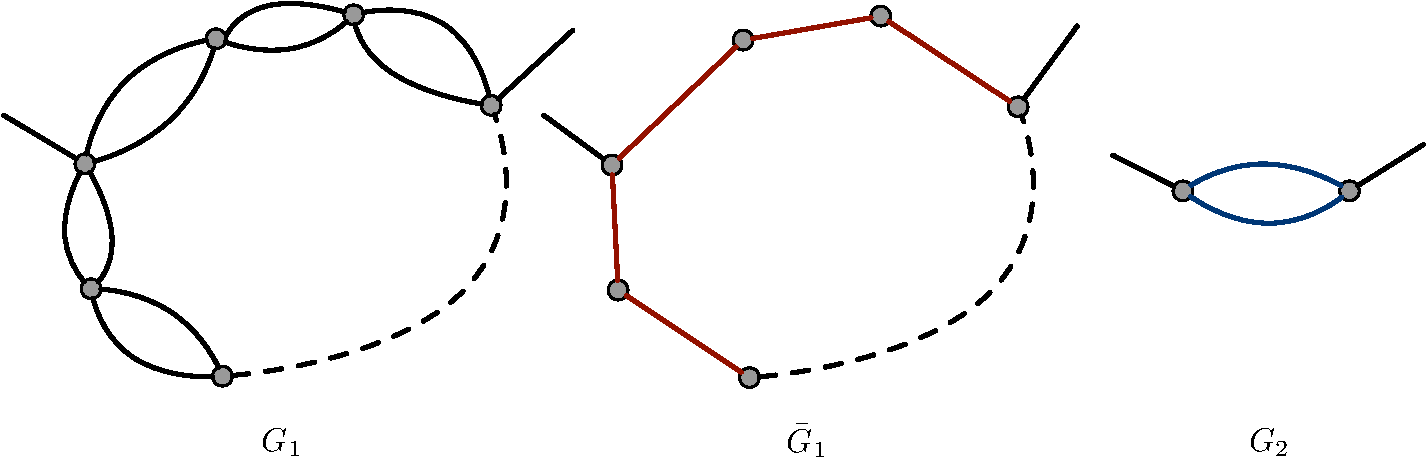
\includegraphics[width=.85\textwidth]{2compress.pdf}
  \end{center}
  \caption{\label{fig:2compress} The figure shows 1 and 2-compression
    $G_1$ and $G_2$ of the graph shown in Figure \ref{fig:simplepd}.(ii). In $\bar{G}_1$ we replace parallel
    edges in $G_1$ by twin edges. }
\end{figure}

We obtain graph $\bar{G}_1$ from $G_1$ by replacing each pair of parallel edges
connecting vertices $u$ and $v$ by a single {\em twin} edge $uv$.
Note that each face in this new graph has length at least 3.
Obtain the 2-compression $G_2$ of
$G$ by contracting degree-2 nodes in $\bar{G}_1$; see Figure
\ref{fig:2compress}. In the following, abusing notation slightly, we
call edges created by contracting vertices in $\bar{G}_1$ {\em
twin} (as their projection in $G_1$ must contain twin edges). Using $G_2$, we will now
identify a certain even {\em cycle} whose dual variable we increase. 
We branch into two
cases. 

\paragraph{$G_2$ is simple.}

We first assume that any pair of vertices is connected by at most 1 edge in $G_2$. 
In this case, Corollary \ref{cor:smallec} implies that $G_2$ has an even cycle $C_2$ 
of length at most $11$. Since $G_1$ does not have a short, simple cycle with even
projection, it follows that $C_2$ must contain at least one twin edge.

We now focus on an edge $uv$ on $C_2$, and let $\bar{P}_1$, $P_1$, and $P$
be its projections in graphs $\bar{G}_1$, $G_1$, and $G$, respectively.  
Following the notational conventions of 
\cite{FJP10}, we say that $P$ is the {\em piece} corresponding to $uv$, and we say $P$ is a \emph{double} piece if $uv$ is a twin edge. 
Note that the piece of a non-twin edge $uv$ is a $u,v$-path whose
internal nodes have degree $2$ in $G[V\setminus X]$.

If $uv$ is a twin edge of $C_2$, then the path $\bar{P}_1$ consists of twin, and non-twin
edges. In turn, a twin edge $u'v'$ on $\bar{P}_1$ projects to a
subgraph of $G[V \setminus X]$ that is induced by two internally vertex
disjoint $u',v'$-paths $S_1$ and $S_2$. Furthermore, concatenating these two
$u',v'$-paths yields an odd cycle. 

In summary, one now sees that
the {\em block-graph} of the projection of twin edge $uv$ of $C_2$ is 
a path in $G[V\setminus X]$. Moreover, the
blocks in this subgraph are odd cycles; see Figure \ref{fig:cycG2} for
an example.

\begin{figure}[b]
  \begin{center}
    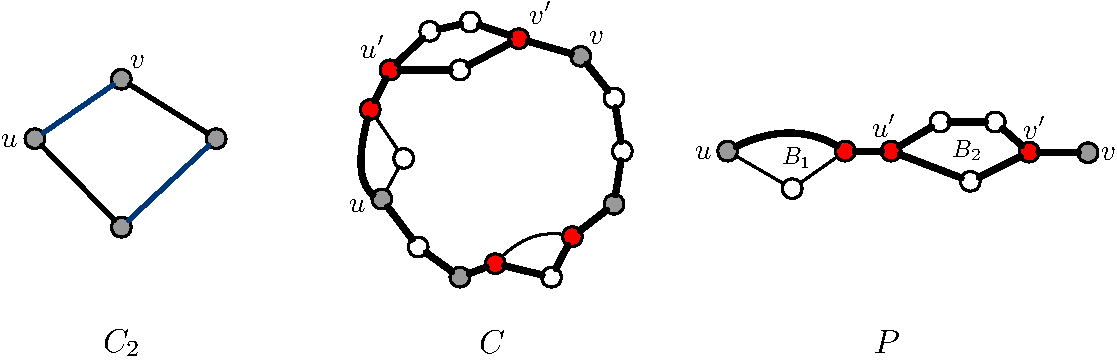
\includegraphics[width=.8\textwidth]{cycG2.pdf}
  \end{center}
  \caption{\label{fig:cycG2}The first two figures show a  short cycle $C_2$ in $G_2$, and its
    corresponding projection in $G$. The right figure above shows the piece
    of twin edge $uv$ of $C_2$. Note the thick edges of cycle $B_2$ above: these
    are type-3 edges.}
\end{figure}

Let us focus on a piece $P$ corresponding to a twin edge $uv$ of
$C_2$. Vertices $w \in V(P)\setminus  \{u,v\}$ have degree $2$ in
$G_1$, or they are {\em cut-vertices} of $P$, and have degree $2$ in
$\bar{G}_1$. In Figure \ref{fig:cycG2} we have coloured such vertices
in red.
In the following, we keep track of the 
{\em slack} in the dual constraint of each vertex $v$ for the current dual feasible
solution for \eqref{lp:d3}:
\[ \bar{c}_v := c_v - \sum_{(C'_1,C'_2) \in \C} a^{C'_1,C'_2}_vy_{C'_1,C'_2}.\]
We now define a {\em canonical} subgraph of each piece $P$. 
This subgraph will be the support of the inequality of \eqref{lp:p3} whose dual variable
we want to increase. The subgraph is induced by a set of vertices 
that we classify as {\em type-1}  
{\em type-2}, or {\em type-3}.

For a non-twin edge
$uv$ of $C_2$ we let all vertices of the corresponding piece $P$ be of type 1. 
Now consider a twin-edge $uv$ of $C_2$. All vertices of $P_1$ are added as type-1. 
Let $u'$ and $v'$ be two neighbouring vertices on $P_1$ that are connected by twin edges 
$e_1$ and $e_2$ in $G_1$ (see Figure \ref{fig:cycG2}). 
Let $S_1$ and
$S_2$ be the paths in $G[V\setminus X]$ corresponding to $e_1$ and
$e_2$, respectively. We let the residual cost $\bar{c}(S)$ of a path $S$ be the
smallest residual cost of any of its internal nodes. 
If the maximum among $\bar{c}(S_1)$ and $\bar{c}(S_2)$ is unique, then let the vertices
of the maximizer be of type 1. Otherwise label $u'$ and $v'$ type-1, and make all internal
vertices of $S_1$ and $S_2$ type-2. We will call the vertices of $S_1$ and $S_2$ together
with $u'$ and $v'$ a {\em type-2 cycle} and call the two $u',v'$ paths \emph{handles} \cite{FJP10} in this case. % Call $u,v$ \emph{end nodes} of the handles and the other nodes

Suppose first that the number of type-2 cycles over all pieces of $C_2$ is
odd. In this case, pick an arbitrary such cycle and label all its internal
vertices type-3. We call the corresponding cycle a {\em type-3 cycle}. For any
$v \in V$, we now let
\[
  a_v = \begin{cases} 
    1 & \mbox{if $v$ is type-1, or type-3}\\
    1/2 & \mbox{if $v$ is type-2}\\
    0 & \mbox{otherwise.}  
    \end{cases}
\]
We claim that the inequality
\begin{equation}\tag{$\circledast$}\label{eq:star} 
  \sum_v a_v^{C_2} x_v \geq 1 
\end{equation}
is part of \eqref{lp:p3}. To see this, let us assume that the number of type-1
vertices is even (the subsequent argument is easily adapted if this number is
odd). Let $\bar{C}^1, \ldots, \bar{C}^{2q}$ be the even cardinality set of all
type-2 cycles over all pieces of $C_2$. Furthermore, for $1 \leq i \leq 2q$,
let $ \bar{S}^i_1$ and $\bar{S}^i_2$ be the internal vertices of the two paths
defining $\bar{C}^i$. Since $\bar{C}^i$ is odd by assumption it follows that
$\bar{S}^i_1$ and $\bar{S}^i_2$ have different parity. By possibly
renumbering, we may therefore assume that the parity of $\bar{S}^{2i}_1$ is
different from that of $\bar{S}^{2i+1}_1$, for all $1 \leq i \leq q$. 

Assume first that there are no type-3 vertices. In this case, we obtain two
even cycles, by adding the set of type-1 vertices to  
\[ Q_j =
\bigcup_{i=1}^q(\bar{S}^{2i}_j \cup \bar{S}^{2i+1}_j), \]  
for $j=1,2$. 
Assume, on the other hand, that there are type-3 vertices, and let $S_1 \cup S_2$ be the
corresponding partition of the internal vertices of the paths defined above. 
We now see that adding the set of type-3 vertices to $Q_j$ yields the superset
of an even cycle, for $j=1,2$. This now completes the argument that \eqref{eq:star} is
part of \ref{lp:p3}.  We will call inequality \ref{eq:star} the \emph{blended inequality} for $C_2$. When $ C$ is a cycle of $G$ or $G_1$, we will also call the inequality $ \sum_{v \in V(C)} x_v \geq 1 $ a blended inequality for $C$.

The algorithm increases the dual variable $y_{\circledast}$ corresponding to
inequality \eqref{eq:star} as much as possible, while maintaining dual feasibility. 
We then add tight vertices to $X$. Note that our definition of $a$ and inequality 
\eqref{eq:star} allows us to maintain the following invariant.

\begin{inva}\label{inva}
  Consider a twin edge $e_1$ and $e_2$ in $C_1$ as defined above, and let $S_1$ and $S_2$
  be the corresponding vertex sets in $G[V\setminus X]$. If $\bar{c}(S_1) \geq \bar{c}
  (S_2)$ before the increase of $y_{\circledast}$ then this will be true also after the
  increase, and until the end of the algorithm's execution. 
\end{inva}

Let $S_1 \cup S_2$ be the set of internal vertices of a type-2 or type-3 cycle. Note that
Invariant \ref{inva} implies that if the dual constraint of some $v_1 \in S_1$ becomes
tight in a step of the algorithm, then there is a vertex $v_2 \in S_2$ whose dual
constraint becomes tight at the same time. For such a tight cycle, we pick exactly two
vertices
$v_1$ and $v_2$ in $S_1$ and $S_2$, respectively, and add them to $X$. We will later refer
to such an addition as a {\em type-2/3 addition}.

\paragraph{$G_2$ is not simple.}

In this case, $G_2$ has two vertices $u$ and $v$ that are connected by at least two edges
$e_1$ and $e_2$. By assumption $\bar{G}_1$ is a simple graph. Thus, at least one of $e_1$
and $e_2$, say $e_1$, is a twin edge. In this case we let $C_2$ be the cycle formed by
$e_1$ and $e_2$ and proceed as above.

\paragraph{When the algorithm terminates.}

The algorithm terminates at the first time when $X$ is a feasible solution to \ect. We
then obtain a minimal feasible solution $\bar{X}$ through a reverse-delete step. 
Suppose that reverse delete considers vertices $v_1$ and $v_2$ that were part of a
type-2/3 addition in the algorithm. Note that if reverse delete decides to remove one of
these vertices, then it will remove both. 

\section{Analysis}

Let $y$ be the final feasible dual solution computed by the algorithm. 
Our goal is to prove that the computed solution is $12$-approximate. 
Following the classic primal-dual argument, it
suffices to show that
\begin{equation}\label{eq:pd}
\sum_{v \in \bar{X}} a^{C'_1,C'_2}_v \leq 12,
\end{equation}
whenever $y_{C'_1,C'_2}>0$. The inequality follows from the argument used in Lemma 
\ref{lem:simplealg} in the case where $C'_1=C'_2=C$ for some even cycle $C \in \C$
(e.g., this is the
case when our algorithm found a simple, short, even cycle in $G_1$).

So let us consider the situation during the algorithm where no such short, simple, even
cycle exists, but where $G[V\setminus X]$ still has even cycles. 
In this case, as described above, our algorithm computes the 2-compression $G_2$ of $G
[V\setminus X]$ and finds a short cycle $C_2$ whose projection $C$ in $G[V\setminus
X]$ contains an even cycle. In the construction of inequality \eqref{eq:star}, the
algorithm selects
type-1, type-2, and type-3 vertices in $C$.
We will show that the sum of the $a$-coefficients of
the internal vertices of $P \cap \bar{X}$ and any one of $u$ and $v$ is at most $1$ if $P$
has no type-3 vertices, and at most 2 otherwise. Inequality 
\eqref{eq:pd} then follows from the fact that at most one piece of $C_2$ has type-3
vertices by construction. 

Consider first the case where $uv$ is a non-twin edge of $C_2$, and recall that its
piece $P$ is a path whose internal vertices have degree $2$. As in the proof of Lemma 
\ref{lem:simplealg}, at most one of the internal vertices of $P$ can be in $\bar{X}$.
Similarly, if
one of $P$'s endpoints is in $\bar{X}$ then none of the internal vertices can be in
$\bar{X}$.

\begin{figure}
  \begin{center}
    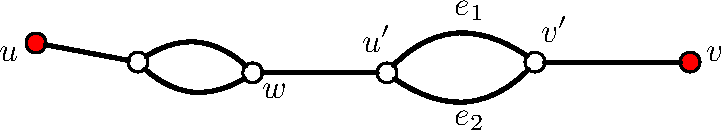
\includegraphics[width=.5\textwidth]{piece.pdf}
  \end{center}  
  \caption{\label{fig:piece} The figure shows the projection $P_1$ of a piece of an
  edge $uv$ on an even
  cycle $C_2$ in $G_2$.}
\end{figure}  

In the remaining part of the proof, we consider a twin edge $uv$ on $C_2$ with
projections $P_1$ in $G_1$, and $P$ in $G[V\setminus X]$; we refer the reader
to Figure \ref{fig:piece} for an example.

\paragraph{Case 1: $P$ has no type-3 vertices.}

As in the proof of Lemma
\ref{lem:simplealg}, $\bar{X}$ has at most one of the internal nodes of $P_1$, and if
there is such a node, then $P$ contains no other node of $\bar{X}$. In this case, 
the sum of $a^{C'_1,C'_2}_v$ over the nodes of $P \cap \bar{X}$ is at most 1.
So suppose that $\bar{X}$ has none of the internal vertices of $P_1$. 

Focus, on a pair of twin edges $e_1$ and $e_2$, connecting vertices $u'$ and
$v'$ of $P_1$, and as before, let $S_1$ and $S_2$ be the vertex sets of the
projections of these edges.  Suppose that the residual cost of $S_1$ is at
least that of $S_2$. Then by Invariant \ref{inva}, and by the way we perform
reverse-delete, $\bar{X}$ contains a vertex from $S_1$
only if it also contains a vertex of $S_2$. If $S_1 \cup S_2$ forms a type-2/3 cycle, then
a stronger condition holds: $\bar{X}$ contains either exactly two vertices $v_1 \in S_1$,
and $v_2 \in S_2$, or $(S_1 \cup S_2)\cap \bar{X}=\emptyset$. 
%Moreover, the piece $P$
%contains at most one type-2/3 cycle with  non-empty intersection with $\bar{X}$. 

Let us first assume that $\bar{X}$ contains
vertices from both $S_1$ and $S_2$. In this case, by the familiar witness cycle
argument, we see that these two vertices are the only vertices in $P \cap
\bar{X}$. If $S_2$ is in the support of \eqref{eq:star} then it must be that
the projection of $e_1$ and $e_2$ forms a type-2 cycle. Thus, the sum of the
$a$-coefficients of the two $\bar{X}$-vertices in $S_1 \cup S_2$ is $1$ in
this case. On the other hand if $e_1$ and $e_2$ do not form a type-2 cycle,
then $S_2$ is not in the support of \eqref{eq:star}, and hence the sum of
$a$-coefficients of vertices in $P$ is at most $1$ in that case as well. 

Let us now assume that for all cycles $S_1 \cup S_2$ of piece $P$, $\bar{X}$
contains at most one vertex from $S_1 \cup S_2$. Thus, if $\bar{X} \cap S_2
\neq \emptyset$ we must have $\bar{X}\cap S_1=\emptyset$ for such a cycle. But
this implies that we must have had $\bar{c} (S_1)>\bar{c}(S_2)$ at the time of
increase, and hence $a(S_2)=0$. 

\paragraph{Case 2: $P$ has type-3 vertices.}

Let $S_1,S_2$ be the vertex set of the type-3 cycle. By the same argument as before, 
$\bar{X}$ contains none or two vertices from $S_1 \cup S_2$. If it contains none, then the
argument of the previous case applies and the sum of $a$ coefficients of $P$ vertices is
at most $1$. Otherwise, $P$ contains exactly these two vertices from $\bar{X}$, and the
$a$ coefficients of $P$ vertices sum to $2$. Since at most one piece of $C_2$ can contain
type-3 vertices, we now obtain the following theorem. 

\begin{theorem}
  The above algorithm is $12$-approximate. 
\end{theorem}

We can get an 11-approximation by using a stronger version of Corollary \ref{cor:smallec}
that is specifically tuned for our application. In the following, let $G_2$ be the
2-compression of a given planar graph $G$. As before, we assume that $G_2$ is 2-connected.

By an abuse of notation, we will say that a cycle of $G_2$ or $G_1$ is even if its projection in $G$ is even.
\begin{corollary}\label{cor:smallec improved}
Suppose that $G_2$ has no face of length 2. Then either \\ (a) it contains an even cycle without twin edges of length at most $11$, or \\ (b) it contains a cycle $C$ that contains a twin edge of length no more than $10$. 
\end{corollary}
\begin{proof} 
% proof
If $G_2$ has parallel edges, one of which is twin, then we get an even cycle with at most 3 pieces.
By Lemma \ref{discharge} we can find adjacent faces $f_1,f_2$ of $G_2$ whose lengths sum
to at most 13. If one of the faces has a twin edge, then the corresponding cycle satisfies
condition (b) above. Otherwise, the union of $f_1$ and $f_2$ contains an even cycle
without twin edges of length at most $11$, and hence condition (a) holds. 
\end{proof}
% intro to 10 apx
One can improve the 11-approximation by noting that tightness in Corollary \ref{cor:smallec improved} only happens in a very specific case. In particular it requires tightness of Lemma \ref{discharge} for $G_2^*$. That is, suppose nodes $v$ and $u$ of $G_2^*$ have degrees summing up to 12 or less. Then either the face $v$, or  face $u$, or the  cycle $C$ consisting of the disjoint union of the face $v$ and the neighbouring face $u$ is even.  If $u$ or $v$ is an even face of $G_2$, then we get an even cycle with 9 or fewer pieces, otherwise $C$ has at most 10 pieces, none of which is twin.  
%For the next part, let us modify which nodes were added to our ECT as follows. We remove any nodes that were not paid for by our blended diamond inequality, and if two internal nodes of a type 2 cycle were selected, we instead choose an end-node of that cycle and declare that that vertex is selected instead. This does not decrease  $\sum_{v \in \bar{X}} a^{C'_1,C'_2}_v $.   Given an edge $uv$ in $G_2$, let $p(u,v)$ denote the piece corresponding to $uv$ in $G$.
Otherwise by the discussion following Lemma \ref{discharge} $G_2^*$ has a particular vertex.  Let us define a notion of what the corresponding face of a particular vertex of $G_2^*$ looks like.
\begin{definition}
Let us call a face $f$ of $G_2$ \emph{particular}, if in $G_2^*$ $f$ has exactly 5 light and 5 heavy neighbours, and they alternate in the clockwise order around $f$. We  also require that at least 4 of the light neighbours of $f_1$ in $G^*$ have degree 3. Further, in $G_2$ edges lying on both $f$ and a  face of length 3 have both endpoints degree 3.
\end{definition}
We state our above observations in the following lemma:
\begin{lemma}\label{improved ec}
  Suppose that $G_2$ has no face of length 2. Then one of the following holds: \\
  (a) The graph $G_2$ contains an even cycle without
twin edges of length at most $10$. \\
(b) The graph $G_2$ contains a cycle $C$ that contains a twin edge of length no more than $9$. \\
(c) The graph $G_2$ contains an even cycle without twin edges of length $11$ that contains exactly 2 faces $f_1$ and $f_2$, and $f_1$ is particular. \\  % Further, $f_1$ has length 10 and $f_2$ length 3. In $G_2^*$ $f_1$ has exactly 5 light and 5 heavy neighbours  and they alternate in the clockwise order around $f_1$. Also, at least 4 of the light neighbours of $f_1$ in $G^*$ have degree 3. Further, in $G_2$ edges lying on both $f_1$ and a  face of length 3 have both endpoints degree 3. \\
(d) The graph $G_2$ contains a particular face $f$ that contains a twin edge.  %In $G_2^*$ $f$ has exactly 5 light and 5 heavy neighbours, and they alternate in the clockwise order around $f$. Also, at least 4 of the light neighbours of $f_1$ in $G^*$ have degree 3. Further, in $G_2$ edges lying on both $f$ and a  face of length 3 have both endpoints degree 3. 
\end{lemma} 
The algorithm for this part will first look for an even cycle with 10 or fewer edges in the 1-compression. Then it will look for an even cycle with 9 or fewer edges in $G_2$. If both previous steps fail to find an even cycle, we then choose an even cycle of $G_2$ that is guaranteed by Lemma \ref{improved ec}. Denote this cycle by $C$ and let $\sum_v a_v^C x_v \geq 1 $ be the blended inequality for $C$. Increment the dual variable for this inequality until a  constraint $\sum_{(C'_1,C'_2) \in \C} a^{C'_1,C'_2}_vy_{C'_1,C'_2} \leq c_v $ of the LP (\ref{lp:d3}) becomes tight. Add newly tight nodes to $X$.  At the end of the algorithm when all even cycles intersect a node of $X$, run a reverse deletion procedure on $X$ to obtain $\bar{X}$. 
\begin{theorem}
  The algorithm described above is a 10-approximation.
\end{theorem}
%That would give us a 10 approximation. Thus we assume that we do not find 2 adjacent faces of $G_2$ whose degrees sum to less than 13. 
%\end{remark} 
% connecting sentence
%We now modify our algorithm to return either an even cycle with 8 pieces or one that is contained in the projection of once of the cases of Lemma \ref{improved ec}.
\begin{proof} 
% 10 apx case a) or b)
To prove that this is a 10-approximation, we will show the set $\bar{X}$ returned by our algorithm satisfies $\sum_{v\in \bar{X}} a_v^C  \leq 10 $. If $C$ is a cycle in the 1-compression with 10 or fewer pieces, then the claim is clear.  Otherwise, let $\bar{X}'$ be obtained from $\bar{X}$ by first removing any nodes not in the support of $a^C$.  Next, while $ \bar{X}'$ contains  an internal node on both handles of a type 2 cycle, we replace the 2 nodes with an end node of one of the handles.  We have $\sum_{v\in \bar{X}'} a_v^C \geq \sum_{v \in \bar{X}} a_v^C$. We now prove $\sum_{v\in \bar{X}'} a_v^C \leq 10$.
%We now prove the 10-approximation as follows. 
If $C$ satisfies case (a) or (b) of Lemma \ref{improved ec},  the 10-approximation follows in the same manner as the previous 11-approximation.  Suppose we are in case (c), denote the vertices of $f_1$ by  $v_1,v_3,v_4 ,.., v_{11}$, and the node of $f_2$ not on $f_1$ by $v_2$.  Let $v_i t v_{i+1}$ be a triangle face sharing an edge with $f_1$ that is not $f_2$. By assumption, this face has odd length in $G$.
\begin{remark}\label{consecutive}
Let $ t v_i v_{i+1} $ be a face of length 3 of $G_2$ which has odd length in $G$ with no twin edges. Let $ v_{i-1} $ be a neighbour of $v_i$, and $v_{i+2}$ a neighbour of $v_i$. Suppose that $v_i $ and $v_{i+1}$ have no other neighbours. Then  $ p(v_{i-1} , v_i ) \cup p(v_i,v_{i+1} ) \cup p(v_{i+1},v_{i+2} ) $  contains fewer than 3 hit nodes; see Figure \ref{b-faceAndLastdnodeAndCon} (iii).
  % Let  non twin edge distinct from $ v_1 v_3 $ , let $ v_i t_i v_{i+1}$  be the triangle face  using $v_i, v_{i+1} $ if each of $v_i, v_{i+1}$ is incident to exactly 3 faces. 
\end{remark}
\begin{proof}
%proof
 Suppose that $ p(v_{i-1} , v_i ) \cup p(v_i,v_{i+1} ) \cup p(v_{i+1},v_{i+2} ) $ contains 3 hit nodes. Let $w$ be the  ``middle" hit node. Then each of $ p(v_{i-1} , v_i ) $ and $ p(v_{i+1},v_{i+2} ) $ contains a hit node besides w. Let $A_w$ be a witness cycle for $w$, and consider the subpath $ Q_w$ of $A_w$ containing $w $ and lying in $ p(v_{i-1} , v_i ) \cup p(v_i,v_{i+1} ) \cup p(v_{i+1},v_{i+2} ) \cup p(v_{i+1},t) \cup p(v_i,t)  $  such a path cannot use nodes of $ p(v_{i-1} , v_i ) \backslash v_i ,p(v_{i+1},v_{i+2} ) \backslash v_{i+1} $  and hence both ends of the path are  $t$ and so $A_w$ is the projection of $t v_i v_{i+1} $. But by assumption this cycle is odd in $G$, which is a contradiction.  
\end{proof} 

%using remark to finish proof
Thus $p(v_{i-1},v_i) \cup p(v_{i},v_{i+1}) \cup p(v_{i},v_{i+1})$ contains at most 2 hit nodes. The remaining 8 pieces have at most 8 hit nodes not counting $v_{i-1},v_{i+2}$, which implies $\sum_{v \in X} a^{C'_1,C'_2}_v x_v \leq 10$.  Case (d) is similar. Let $G'$ be the graph obtained from $G$ by deleting the interior nodes of one handle of a type 3 cycle. Let the even cycle be $v_1 v_2 ... v_{10}$, and $v_i,t,v_{i+1}$ be a triangle face of $G_2$. By remark \ref{consecutive} the union  $p(v_{i-1},v_i) \cup p(v_{i},v_{i+1}) \cup p(v_{i},v_{i+1})$ contains at most 2 hit nodes. The remaining 7 pieces with $v_{i-1},v_{i+2}$ removed contain at most 7 hit nodes,  which again proves $\sum_{v \in X} a^{C'_1,C'_2}_v x_v \leq 10$. 
 \end{proof}
 %introducing the 9 apx
 By being a bit more careful in our book-keeping, we can get a 9-approximation.
 
 \begin{lemma}\label{light+}  \cite{JV13} 
A planar multigraph $ G=(V,E)$ where every vertex has  at least 3 neighbours embedded with no face of length 2 contains  an  edge $uv$ such that one of the following is true: \\
1) $u$ has degree 3 and if $v$ has degree more than 6 it has degree at most $2a_1 + a_2 + 2c +d $ with $ 6-(a_1+a_2) -1.5c -d -b > 0 $. Here $ a_1 $ is the number of neighbours $w $ of degree 3 for which  the next neighbour of $v$  in the clockwise order is heavy and $a_2$ is the number of other neighbours of degree 3.  %  of $G$ that contain $vw$ are triangles, $a_2$ is the number of neighbours $w$ of $v$ of degree 3 for which not both faces of $G$ that contain $uw$ are triangles 
$c$ is the number of neighbours of degree 4 or 5. $b$ is the number of faces of length 4 or more containing $v$ and both a light and heavy neighbour of $v$ in $G$. $d$ is the number of heavy neighbours $w$ of $v$ whose such that the next clockwise neighbour of $v$ is also heavy; see Figure \ref{Triangulating}. \\ % $b$ is the number of faces of  
2) $  \text{deg}(u) + \text{deg}(v) \leq  11. $ % \text{max} (10, 11 -b -c_2 ) $ where $c_2$ is the number of light neighbours of $v$ for which either the next  (in the clockwise order) is light. \\

\end{lemma}
\begin{proof}
%(of part not in \cite{JV13})
%proof up to a reasonable length
 If $G$ contains  2 adjacent light neighbours, we are done. Otherwise, let $G'$ be a triangulation of $G$ by drawing edges between heavy vertices. Note that this is possible, since any face of length four or more contains 2 heavy nodes, and we can add an edge between them.  Just as in \cite{JV13}, by maximality of our triangulation $v$ cannot have 2 consecutive light neighbours in $G'$.

\begin{figure}[h]
    % 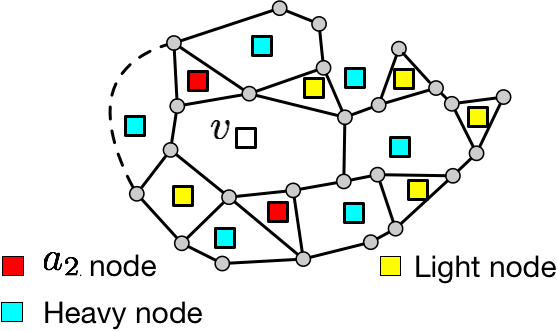
\includegraphics[scale=0.28]{PreTriang.png}
  \begin{center}
   % \hspace*{.2\textwidth}
    %  \begin{subfigure}[t]{.48\textwidth}
     %   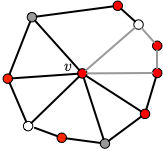
\includegraphics[width=0.48\textwidth]{UntriangulatedDual.png}
      %   \end{subfigure} 
    %\hspace*{-.18\textwidth}
     % \begin{subfigure}[t]{0.48\textwidth}
      %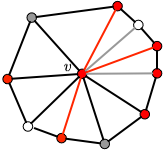
\includegraphics[width=0.48\textwidth]{TriangulatedDual.png}
    %\end{subfigure}
        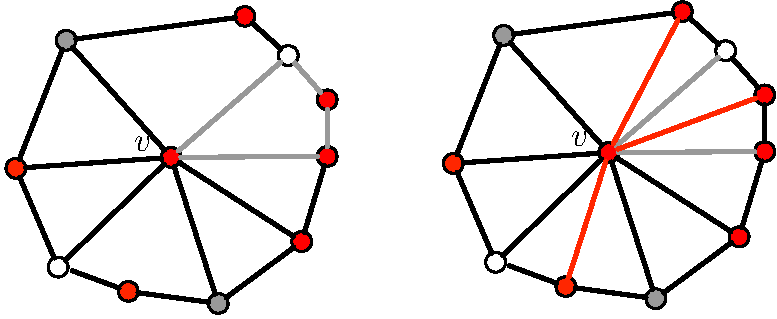
\includegraphics[width=0.48\textwidth]{UntriangulatedAndTriangulatedDual.pdf}
  \caption{\label{Triangulating} Example of a graph $G$ and edges added in obtaining $G'$. The grey, white, and red nodes are $a_2$, other light neighbours of $v$, and heavy nodes, respectively. The grey face is a $b$-face. } 
  \end{center}
  %  \caption{From left to right: Depiction of the $G^*$ with various nodes of $G$,  $G$, and the result of triangulating $G$.}
\end{figure}

 In the proof of Lemma \ref{discharge} it was shown there exists an edge $uv$, where $v$ is a vertex with positive charge such that either \\
 1) $u$ has degree 3 and $\text{deg}_{G'}(v) \leq 10$, or \\
 2) $\text{deg}_{G'}(u)+ \text{deg}_{G'}(v) \leq 11$.
%Let $f'$ be the number of non heavy neighbours of $v$ in $ G' -G $.
%logical spot to break up long paragraph

We claim $v$ has degree at least  $2a_1 +2a_2+2c+d +b  $ in $G'$. First, let $f_1, f_2,.., f_b$ be the $b$-faces of $G$ that is the faces that $b$ is counting. Let $E'$ be the set of edges of $\delta_{G'} (v)$ contained in the interior of some $f_i$ and $E''$ be the $d$-edges, that is the edges whose endpoint other than $v$ is counted by $d$.  In any $f_i$ one neighbour $u$ of $v$ is light and the other $u'$ is heavy. Therefore $uu'$ is not an edge of $G'$. So $ \delta_{G'}(v) $ contains an edge in the interior of $f_i$. It thus suffices to prove that $ | \delta_{G'}(v) \backslash E' \backslash E'' | \geq  2a_1 +2a_2+2c$.  We claim that in $ (G' \backslash E' ) \backslash E'' $ there are no consecutive light neighbours of $v$. Assume for a contradiction that there were 2 such neighbours $w,w'$ with $w'$ the next neighbour after $w$ in $ (G' \backslash E' ) \backslash E'' $ in the clockwise order about $v$. Suppose that there is a $d$ neighbour $u'$ between $w$ and $w'$ in $G'$, let $u''$ be the last such $d$ neighbour of $ v $ before $w'$ in the clockwise order. Then there is a heavy non $d$ -neighbour $q$ of $v$ in $G$  which lies between $ u''$ and $w' $.  So henceforth we assume that no $d$-neighbours lie between $w$ and $ w'$ in the clockwise order about $v$ in $G'$.  

%good spot to break up??
Let $u'$ be the previous neighbour before $w'$ in $G'$. % Since $u'$ is heavy and $u'$ and the next neighbour in the clockwise order is light, $u' \notin E''$ 
%I could not figure out how to best explain this simple fact
Assume $vu \in  E'$ so $u' \in f_j$ for some $f_j$. Note  $f_j$ contains 2 consecutive neighbours of $v$ in $G$ and contains the edge $vu$ in its interior, and $u$ lies between $w,w'$ in the clockwise order. So the neighbours of $v$ in $f_j$ lie between $w,w'$ in the clockwise order. So $f_j$ must contain  $vw$ or  $ vw'$.  Since one of them is light, that neighbour must be $w$ or $w'$.  Let  $w''$ be the  one of $w,w'$ contained in $f_j$ and let $u''$ be the other neighbour of $v$ in $G$, then $u''$ lies between $w,w'$ in the clockwise order, which is a contradiction.  %Since both $w,w'$ are neighbours of $v$ in $G$,  $w'', u''$ or $ u'',w'' $ are consecutive.  %  the case that $u''$ is a $d$-neighbour was already addressed. %since $u$ is a  and hence  and light neighbours of $v$ in $f_j$ respectively, then $u''$ lies (as a neighbour) clockwise of $w$ and counterclockwise of $w'$ and further $u''$ lies counterclockwise of $u''$ and hence $f_j$  contains $vw'$ (rather than $vw$ ).  This implies that $v u' \notin E'' $ but $vu'$ lies between (in the clockwise order about v) $w,w'$ which is a contradiction
Hence there are no 2 consecutive light neighbours.  
% seemed like a good point to break up the proof
Since each light edge is preceded and followed by a heavy edge hence $ |\delta_{G'}(v) \backslash E' \backslash E'' | \geq  2a_1 +2a_2+2c$. Calculating charge thus gives us $ 6-(a_1+a_2) -1.5c -d -b > 0 $.
\begin{figure}[h]
\begin{center}
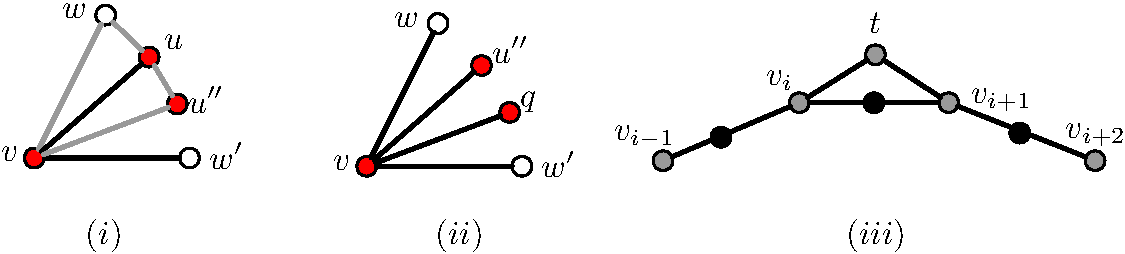
\includegraphics[width=0.8\textwidth]{b-faceAndLastdnodeAndConhit.pdf}
\caption{In (i), $w''=w$. Since $w,u$ are consecutive in $G$, $u''$ must lie before $w'$. In (ii), if there is a heavy node between $w,w'$ then there is a non-$d$ neighbour heavy node. In (iii), since $t v_i v_{i+1}$ is odd and $v_i, v_{i+1}$ have exactly 3 neighbours, the hit node on $v_iv_{i+1}$ cannot have a witness cycle. \label{b-faceAndLastdnodeAndCon}}
        \end{center}
\end{figure}
%Now suppose that  $\text{deg}_{G'}(u)+ \text{deg}_{G'}(v) \leq 11$. Now each $c_2$ neighbour must be followed in the clockwise order  by a heavy neighbour in $G'$ and each $b$-face $f_j$ contains an edge of $E(G') \backslash E(G)$ in it's interior. Thus  $  \text{deg}(u) + \text{deg}(v) \leq 11 -b -c_2 $.
\end{proof}
%\p definition paragraph
When  $G$ and $v\in G$ are specified we will denote by $a_1,a_2,b,d,c$ neighbours as those neighbours of $v$ counted by $a_1,a_2,b,d,c$v respectively and a $a_1,a_2,b,d,c$  edge as an edge between $v$ and a $a_1,a_2,b,d,c$ neighbour respectively.
%
\begin{remark}\label{light+r}
In case 1) of lemma \ref{light+} we have that $v$ has degree at most $ 10 - a_2 -2 \lfloor 0.5c \rfloor -d -2b$
\end{remark}
\begin{proof}  Using same variables as Lemma \ref{light+}, $ 6 > (a_1+a_2) +1.5c +d +b $ so $ 5 \geq \lfloor (a_1+a_2) +1.5c +d +b \rfloor $ so  $ 5-(a_1+a_2) - \lfloor 1.5c \rfloor -d -b \geq 0$ which implies $  10 \geq 2(a_1+a_2) +2c +2 \lfloor 0.5c \rfloor +2d +2b \geq \text{deg}(v)  +a_2 +2 \lfloor 0.5c \rfloor +d +2b  $.
\end{proof}
%
\begin{lemma}\label{even reduced+}
We can find a cycle $C$ of $G_2$, even in $G$ such that either: \\
1)  $C$ is the union of 2 faces $f_1$ and $f_2$ of $G_2$ with, $f_1$ length 3 and at most  $ \text{max}(9, 11- a_2 -2 \lfloor 0.5 c \rfloor -d  -b $) pieces.   Where $ a_2, c ,d ,b $ are as in Lemma \ref{light+}  for $G_2^*$ with $v=f_1$  and $C$ is disjoint from the interior of any double piece. \\ 
2) $C$ has at most 9 pieces and is disjoint from the interior of any double piece. \\
3) $C$ has at most $10- a_2 -2 \lfloor 0.5 c \rfloor -d  -b $  pieces. One piece may be double. \\
4) $C$ has at most 7 pieces. \\
Where for 1),2) $a_1,a_2, c, d, b ,c_2$ are as in Lemma \ref{light+} with  $ v=v_2$  $u=f_1$ in the dual of $G_2$.
\end{lemma}
\begin{proof}
%\p proof
 Apply Lemma \ref{light+} to $G_2^*$.  In case 1) of Lemma \ref{light+}  we find a node $u$ of degree 3 adjacent to a node $v$ of degree at most $10-a_2-2\lfloor 0.5 c \rfloor -d -b$  in $H^*$. Here $a_2,c,d,b$ are as in Lemma \ref{light+}. Let $f_1 , f_2$ be the faces corresponding to $v,u$ in G if $f_1$ or $f_2$ is even such an even cycle satisfies the conditions of out lemma. Otherwise, $f_1 \cup f_2$ is an even cycle in G with at most  $11- a_2 -2 \lfloor 0.5 c \rfloor -d  -b $ pieces. Case 2) is similar.
\end{proof}

\begin{proof} 
% \p breaking proof into cases and case 1)
Let us consider each case of Lemma \ref{even reduced+}. 

Case 1). If $C$ has fewer than 9 pieces we are done. Otherwise let $v_1, v_2, .., v_l$ be the cycle $C$ in $G_2$, with $v_1, v_2, v_3$ vertices belonging to a triangle face of $G_2$. We denote: \begin{equation}
    p'(v_i,v_j) = \begin{cases} 
    \cup_{u=i}^{j-1} p(v_u,v_{u+1}  ) \ \ \ \text{if} \ \  i <j \\
    \cup_{u=j}^{l} p(v_u,v_{u+1} ) \cup \cup_{u=1}^{i-1} p(v_u.v_{u+1}  ) \ \ \text{otherwise}
    \end{cases}
\end{equation} 
Where $ v_{l+i} = v_i $ in above equation. 

%\p case 1a
Case 1a). Vertices $v_1, v_2$ are both incident to 3 faces of $G_2$. We claim that there are at most 3 hit nodes in $p(v_l,v_1) \cup p(v_1, v_2) \cup p(v_2,v_3) \cup p(v_3,v_4)$.
Assume not then each of $p(v_l,v_1) , p(v_1, v_2) , p(v_2,v_3) , p(v_3,v_4)$ contains a hit node, and one of $p(v_2,v_4) \backslash \{v_2 \} , p(v_l,v_2) \backslash \{v_2 \}$  contains 2 hit nodes. By symmetry assume $p(v_2,v_4) \backslash \{v_2 \}$ contains 2 hit nodes. Let $u$ be the node on $p(v_2,v_4) \backslash \{ v_2 \} $  closest to $ v_2$. Now consider the witness cycle $C_u$ of $u$ and consider a subpath $P$ of $ C_u$ lying in $  C $ and let $P'$ be the portion of $P$ starting at $u$ not headed towards $v_2$ $P'$ cannot go to $v_4$ since $p(v_2,v_4) \backslash \{v_2 \}$  contains 2 hit nodes $ p(v_3,v_4) \backslash v_3 $ contains a hit node. So after reaching $v_3$ $P'$ must head towards $ v_1 $ since $p(v_l,v_1) , p(v_1, v_2)$ each contain a hit node $P'$ hits another hit node besides $u$ which is a contradiction.
Let $ f_1,f_2 , a_1, a_2, b,c , d $ be as in lemma \ref{even reduced+}. So we have that $ l \leq 11- a_2 -  2 \lfloor 0.5 c \rfloor -d -2b $  if $l \leq 10 $ then % since each piece is single there are at most 5 nodes on $ ( \cup_{i=5}^l p(v_{i-1},v_i )  ) \backslash v_5,v_l $, and 
since there are at most 3 nodes on $p(v_l,v_1) \cup p(v_1, v_2) \cup p(v_2,v_3) \cup p(v_3,v_4)$  there are at most 9 nodes on $C$. So $a_2 +  2 \lfloor 0.5 c \rfloor +d +2b \leq 1 $

From $l \leq 2a_1+a_2+2c+d$  we get $a_1 \geq 4$ with 3 of the $a_1$ edges not being $v_1v_3$.  Let $ v_r v_{r+1}, v_w v_{w+1} $ be the next and previous $a_1$ edges from $ v_1, v_2 $ on $C$ in the clockwise order and let $ v_k v_{k+1}$ be the remaining $a_1$ edge so $ \{ v_{k-1}v_{k}, v_{k} v_{k+1}, v_{k+1} w_{k+2} \} \cap\{ v_lv_1, v_1v_2,v_2v_3, v_3v_4 \} = \emptyset$ by remark \ref{consecutive} we get 
$ p'( v_{k-1}, v_{k+2} ) \cup p'( v_l , v_ 4 ) $ contains at most 5 hit nodes.
 Since $C \backslash p'( v_{w-1}, v_{w+2} ) \cup p'( v_l , v_ 4 ) $ is contained in 4 pieces we get that $C$ contains at most 9 hit nodes. See Figure \ref{case1}.
 
%\p case 1b)
 Case 1b). Now suppose that one of $v_1, v_3$ is incident to more than 3 faces of $G_2$. Recall  $ l \leq 11- a_2 -2 \lfloor 0.5 c \rfloor -d  -b , 2a_1+a_2+2c+d +1  $.  If $l \leq 9$ we are done otherwise so $c \leq 1, \ \ a_2+b+d \leq 1$  $ a_1 \geq 3 $
 %so either i) $a_1 \geq 4$ % or ii) $a_1=3, \ \  a_2+d \geq 1 $ 
%In case i) 
Thus we can find an $a_1$ edge $ v_r v_{r+1}$  distinct from $v_1 v_3$ that is not proceeded or followed by a $c$ edge. Since  one of $v_1, v_3$ is incident to more than 3 faces of $G_2$ either one of $ v_l v_1 , v_3 v_4$ is an $a_2$ or $ c $ edge or one of $ v_1, v_3$ is a b face in $G_2^*$ which implies that neither $v_r   $ or $v_{r+1}$ can be a b-face  in $G_2^*$ . nor can $v_{r-1} v_r$ be an $a_2$ edge. Combined with $ v_r v_{r+1}$ is an $a_1$ edge we get that $v_r,v_{r+1}$ both have exactly 3 neighbours and by remark \ref{consecutive}  $p(v_{r-1}, v_{r+2} )$ contains at most 2 hit nodes and hence $C$ has at most 9 hit nodes. 

%case 2
Case 2).  A 9-approximation is immediate. 

% case 3
Case 3). %Let $C_1$ be the result of taking only the bottom handle of each (and cut nodes and end nodes) piece of $C$. Since every hit node $v'$ on a top handle except the one on the special cycle (if it exists) is either not paid for, or appears as a pair $v',w'$ where $w'$ is on the bottom handle and the coefficients of $ v',w' $ in our blended diamond inequality are both 1/2, it suffices to prove that $C_1$ contains at most 8 hit nodes. 
Let $G'$ be obtained from $G$ by deleting the internal vertices of one handle of a type 3 cycle of our blended inequality if our inequality has a type 3 cycle, otherwise set $G'=G$. Denote the 2-compression of $G'$ by $G'_2$.
Denote $m(u,v) =p(u,v) \cap G'$ and $m'(u,v)=p'(u,v) \cap G'$.   Where the edges of $C$ in $G_2$ are $v_1,v_2,..,v_l$ note that if $v_i,v_{i+1} , t_i$ is a face of length 3 in $ G'_2$ then $ v_i v_{i+1}$ is a single piece in $G'$ and remark \ref{consecutive} holds for $m'(v_{i-1},v_{i+2})$. From $l \leq 2a_1 + a_2 + 2c +d $
One can check that either \\
i) $a_1 \geq 4 $   $ c \leq 1, \ \ \ b=d=0 $, or \\ $ l \leq 9 $,   $a_2+ 2 \lfloor 0.5c \rfloor +d +b  \leq 1 $.

\begin{figure}[h]
\begin{center}
    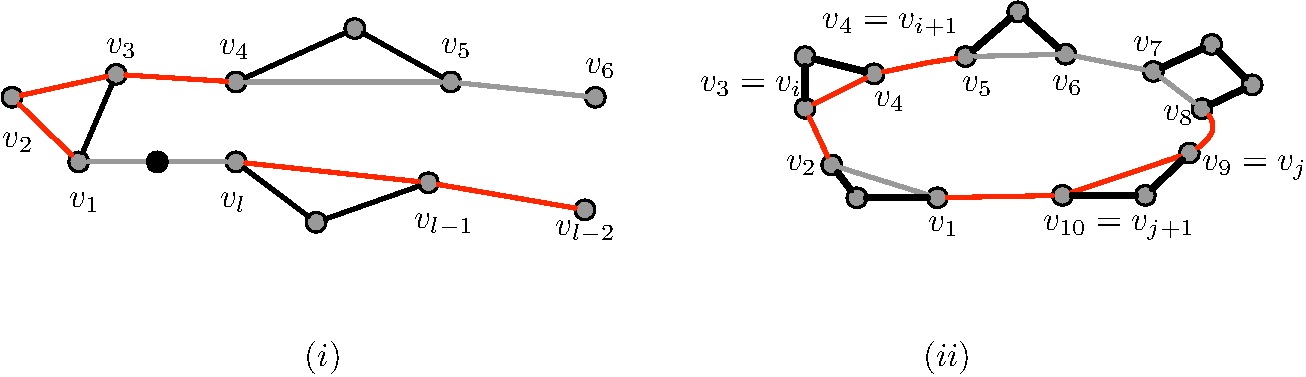
\includegraphics[width=0.85\textwidth]{evenCase1AndCase3a).pdf}
    \caption{\label{Case1nCase3a} (i) shows case 1 and (ii) shows case 3a). }
\end{center}

\end{figure}
%\p case 3a)
Case 3a). We have $b = \lfloor 0.5c \rfloor = d = a_2 =0$. Then there are at least 4 $ a_1  $ edges and since $b=0$ each endpoint of an $a_1$ edge $v_i v_{i+1}$ has exactly 3 neighbours. Thus we can find 2 $a_1$ edges $ v_i v_{i+1} , v_j v_{j+1}$ with $i \neq j-2,j+2$.  Hence $m'(v_{i-1},v_{i+2} )$  , $m'(v_{i-1},v_{i+2} )$ each contain at most 2 hit nodes and hence $C_1$ contains at most 8 hit nodes. 

%\ case 3b
Case 3b).  We have $ b+d + a_2 + 2\lfloor 0.5c \rfloor \ =1 $ and $C_1$ has 9 pieces. Here we wish to show there is an $a_1$ edge with both endpoints having exactly 3 neighbours. If $b=1$, $a_2=d=0$ and from $l \leq 2a_1 + a_2 + c +d $  we get  there are at least 3 $a_1$ edges and the endpoints and thus for at least 1 $a_1$ edge $v_iv_{i+1}$ $v_i, v_{i+1}$  both (since they are not $b$ nodes ) have 3 neighbours.   If $d=1$ then $a_1 \geq 2$ and the endpoints of any $a_1$ edge have exactly 3 neighbours, since they are not $b$ nodes.  

%case 4
Case 4). Our even cycle $C$ has fewer than 7 pieces, then our inequality will count at most 8 hit nodes.
\end{proof}








\bibliography{main}
\bibliographystyle{plain}
\end{document}
